\documentclass{article}

% if you need to pass options to natbib, use, e.g.:
% \PassOptionsToPackage{numbers, compress}{natbib}
% before loading nips_2018

% ready for submission
\usepackage[final]{nips_2018}

% to compile a preprint version, e.g., for submission to arXiv, add
% add the [preprint] option:
% \usepackage[preprint]{nips_2018}

% to compile a camera-ready version, add the [final] option, e.g.:
% \usepackage[final]{nips_2018}

% to avoid loading the natbib package, add option nonatbib:
% \usepackage[nonatbib]{nips_2018}

\usepackage[utf8]{inputenc} % allow utf-8 input
\usepackage[T1]{fontenc}    % use 8-bit T1 fonts
\usepackage{hyperref}       % hyperlinks
\usepackage{url}            % simple URL typesetting
\usepackage{booktabs}       % professional-quality tables
\usepackage{amsfonts}       % blackboard math symbols
\usepackage{nicefrac}       % compact symbols for 1/2, etc.
\usepackage{microtype}      % microtypography
\usepackage{graphicx}

\usepackage{subcaption}

\title{Project Milestone}

% The \author macro works with any number of authors. There are two
% commands used to separate the names and addresses of multiple
% authors: \And and \AND.
%
% Using \And between authors leaves it to LaTeX to determine where to
% break the lines. Using \AND forces a line break at that point. So,
% if LaTeX puts 3 of 4 authors names on the first line, and the last
% on the second line, try using \AND instead of \And before the third
% author name.

\author{M.P.Ross}

\begin{document}

\maketitle

\begin{abstract}
Multimessenger astronomy using gravitational waves require low latency event classification and localization. Previous studies have studied searching for binary coalescence waveforms using machine learning and found that Deep Neural Networks were required to get accurate results. I'm studying applying machine learning to searching for supernovae events and whether these act differently than binary coalescence events.
\end{abstract}

\section{Introduction}
Gravitational waves (GW) are oscillations in space time which are emitted by changing mass quadrupole moments. The only sources that are thought to emit these at measurable amplitudes are cataclysmic astrophysical events including binary neutron star mergers, binary black hole coalescence, and core collapse supernovae. The LIGO/Virgo collaboration has measured GW from multiple binary black hole coalescence and one binary neutron star merger using 4 km long L-shaped interferometric observatories, located in Hanford, WA, Livingston, LA, and Pisa, Italy. The GW are observed by measuring the differential strain along the observatories two arms. Having two or more distant detectors allows us to triangulate the source's location in the sky. 

GW from these events are emitted slightly before any light. Subsequently, one of the goals of our observations is to alert optical telescopes to point towards the source before the light arrives to allow for so called multimessenger astronomy. To achieve this, we need to analyze the strain channel with the smallest latency possible. Additionally, some of these events are buried beneath instrumental noise so complex algorithms are needed to extract them. Currently, the analysis consists of matched filtering or looking for any coherent burst in a set of detectors. Both of these methods are computationally intensive and increase the time between arrival and detection. Machine learning has gained attention lately as a possible alternative to achieve low latency detections. Previous studies have focused on binary coalescence signals as they are the most probable event types (and due to the fact that we've already measured a collection of them) [2, 3]. I'm applying machine learning to supernovae signals which, although they have vastly different waveforms than binary coalescence, should behave similarly under machine learning.

\section{Synthetic event creation}
Due to the lack of true measurements of gravitational waves from core collapse supernovae, to train an algorithm one needs to create a synthetic data set. To make the data as realistic as possible, I took a set of real strain data from the observatories which does not contain any known GW events (this series is referenced later as noise) and injected theoretical supernovae waveforms. The noise data was obtained from the LIGO Open Science Center (https://www.gw-openscience.org/about/) and the waveforms were calculated by the GW theory group at the Max Planck Institute (https://www.mpa-garching.mpg.de/177514/Gravitational-Waveform-Catalog).

To cover a wide range of waveform types and noise conditions, I generated a set of 866 one second long time series half of which had a waveform injected and the other half only containing noise. The noise for each data series was drawn with a random beginning time from the same 1000 second noise time series. For the data sets that contain an injection, a waveform was drawn randomly from a set of 136 and placed at a random time within the one second long noise time series. To begin, the injected waveforms were set to have a large signal to noise ratio to make them easy to see by eye. Below is an example of a time series with and without the injected signal and it's corresponding power spectral density (PSD).

\begin{figure*}[h!]
    \centering
    \begin{subfigure}[t]{0.5\textwidth}
        \centering
        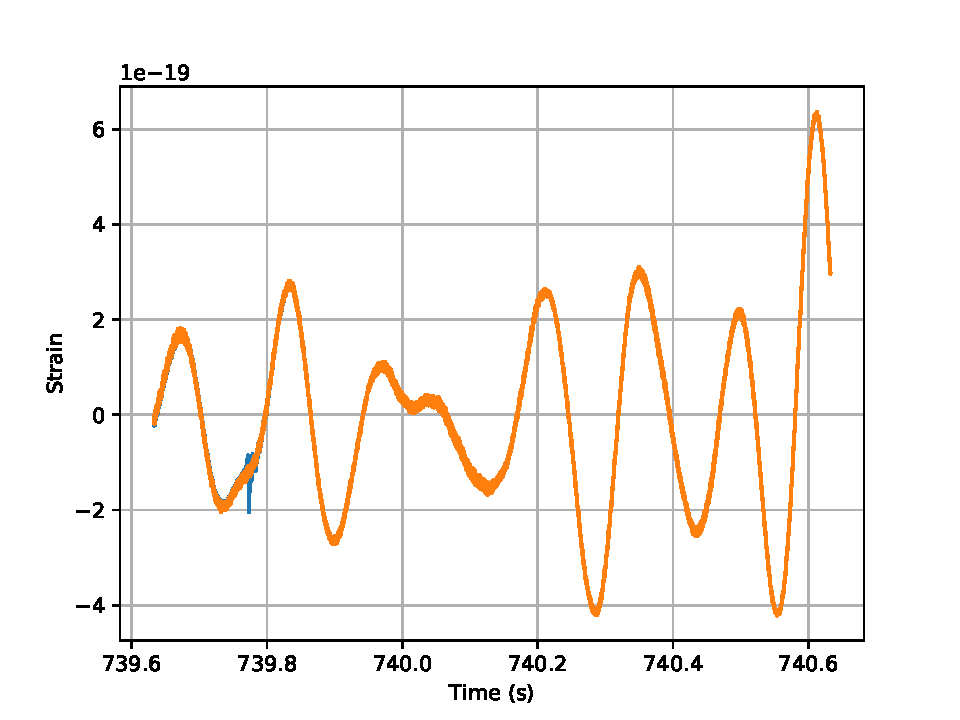
\includegraphics[height=2in]{TimeSeries.pdf}
    \end{subfigure}%
    ~ 
    \begin{subfigure}[t]{0.5\textwidth}
        \centering
        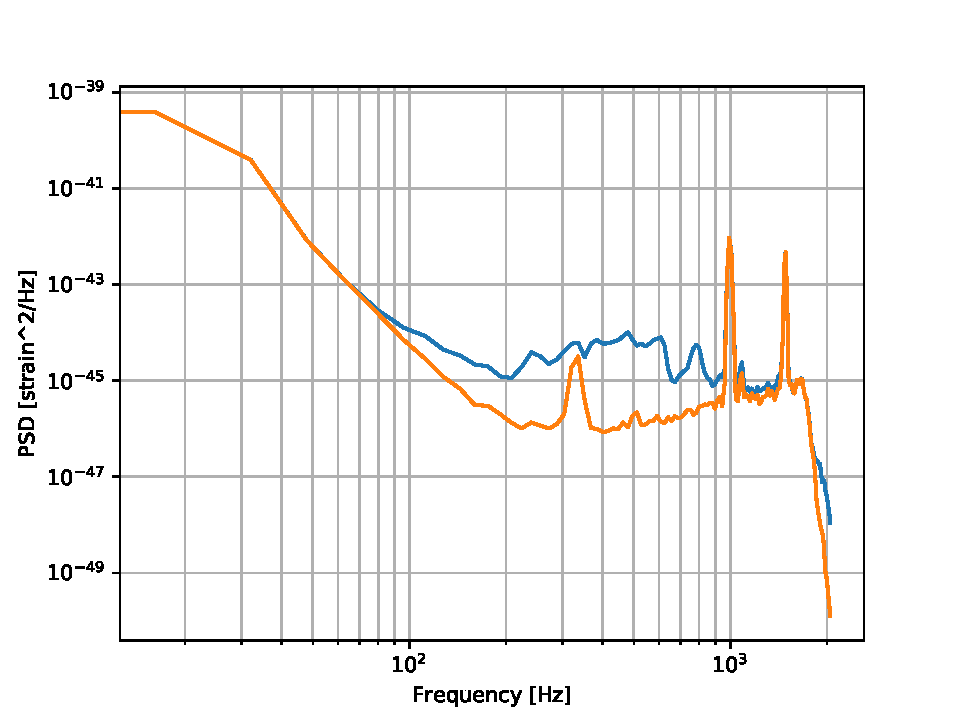
\includegraphics[height=2in]{PSD.pdf}
    \end{subfigure}
    \caption{Time series (left) and power spectral density (right) of a selected synthetic data set with orange being the noise and blue showing the injected waveform. }
\end{figure*}

\section{First attempt classifier}
As a first attempt at classifying the events, I wrote a logistic regression with gradient descent optimization which seemed to work but was taking quite a while to converge. After finding that my algorithm was taking longer than desired, I decided to use the scikit-learn logistic regression which was a significant speed up. 

With a working classifier, I split the data into a training set of 434 data series (half noise, half with signal) and a testing set of 432 series. The first experiment I conducted using these sets and classifier was to compare the performance difference between training on the time series and on the PSD. Intuitively one would expect training on the PSD to perform better since the differences between signal and noise are more pronounced. Additionally, the PSD is independent of when the injected signal happens and will be almost identical for injections using the same waveform. Another added benefit is that it reduces the data set dimensions from 4096 to 129 which clearly speeds up the computations. The results of this test, shown below, matched intuition and the classifier trained and tested on the PSDs was 1.85\% more accurate than the algorithm using the time series.

\begin{center}
\begin{tabular}{ c | c | c }
  & Training Accuracy & Testing Accuracy \\ 
  \hline
  \hline
 Time Series & 100\% & 97.92 \% \\  
 \hline
 PSD & 100\% & 99.77 \%
\end{tabular}
\end{center}

\section{Future investigations}

The next immediate step for this project is to expand my data set. Specifically, to make larger data sets with differing signal to noise and to use these to study the performance of logistic regression at varying SNR. This algorithm would mainly find real world usefulness at low SNR since high signal events can be spotted easily using simple methods such as a local power thresholds. 

With this framework I can then begin to investigate other methods with the goal of comparing the performance of a neural network with simpler algorithms. In Ref. 3, George and Huerta found that simple algorithms like Logistic Regression and Support Vector Machines were no better than chance at finding binary coalescence signals while their Deep Neural Network was close to 100\% accurate. I find this result surprising and want to investigate whether I find similar behavior with supernovae waveforms and at what SNR simple methods begin to fail.

\section*{References}

\medskip

\small

[1] Gossan, S.E., Sutton, P., Sutver, A., Zanolin, M., Gill, K., \ \& Ott, C.D\ (2016) Observing gravitational waves from core-collapse supernovae in the advanced detector era. {\it Phys. Rev. D} {\bf 93}, 042002

[2] George, D., \ \& Huerta, E.A\ (2018) 
Deep Learning for real-time gravitational wave detection and parameter estimation: Results with Advanced LIGO data. {\it Physics Letters B} {\bf 778}

[3] George, D., \ \& Huerta, E.A\ (2018) Deep neural networks to enable real-time multimessenger astrophysics. {\it Phys. Rev. D} {\bf 97}, 044039

\end{document}